\section{Method}
\label{sec:method}

\begin{figure*}[t]
    \centering
    \centering
    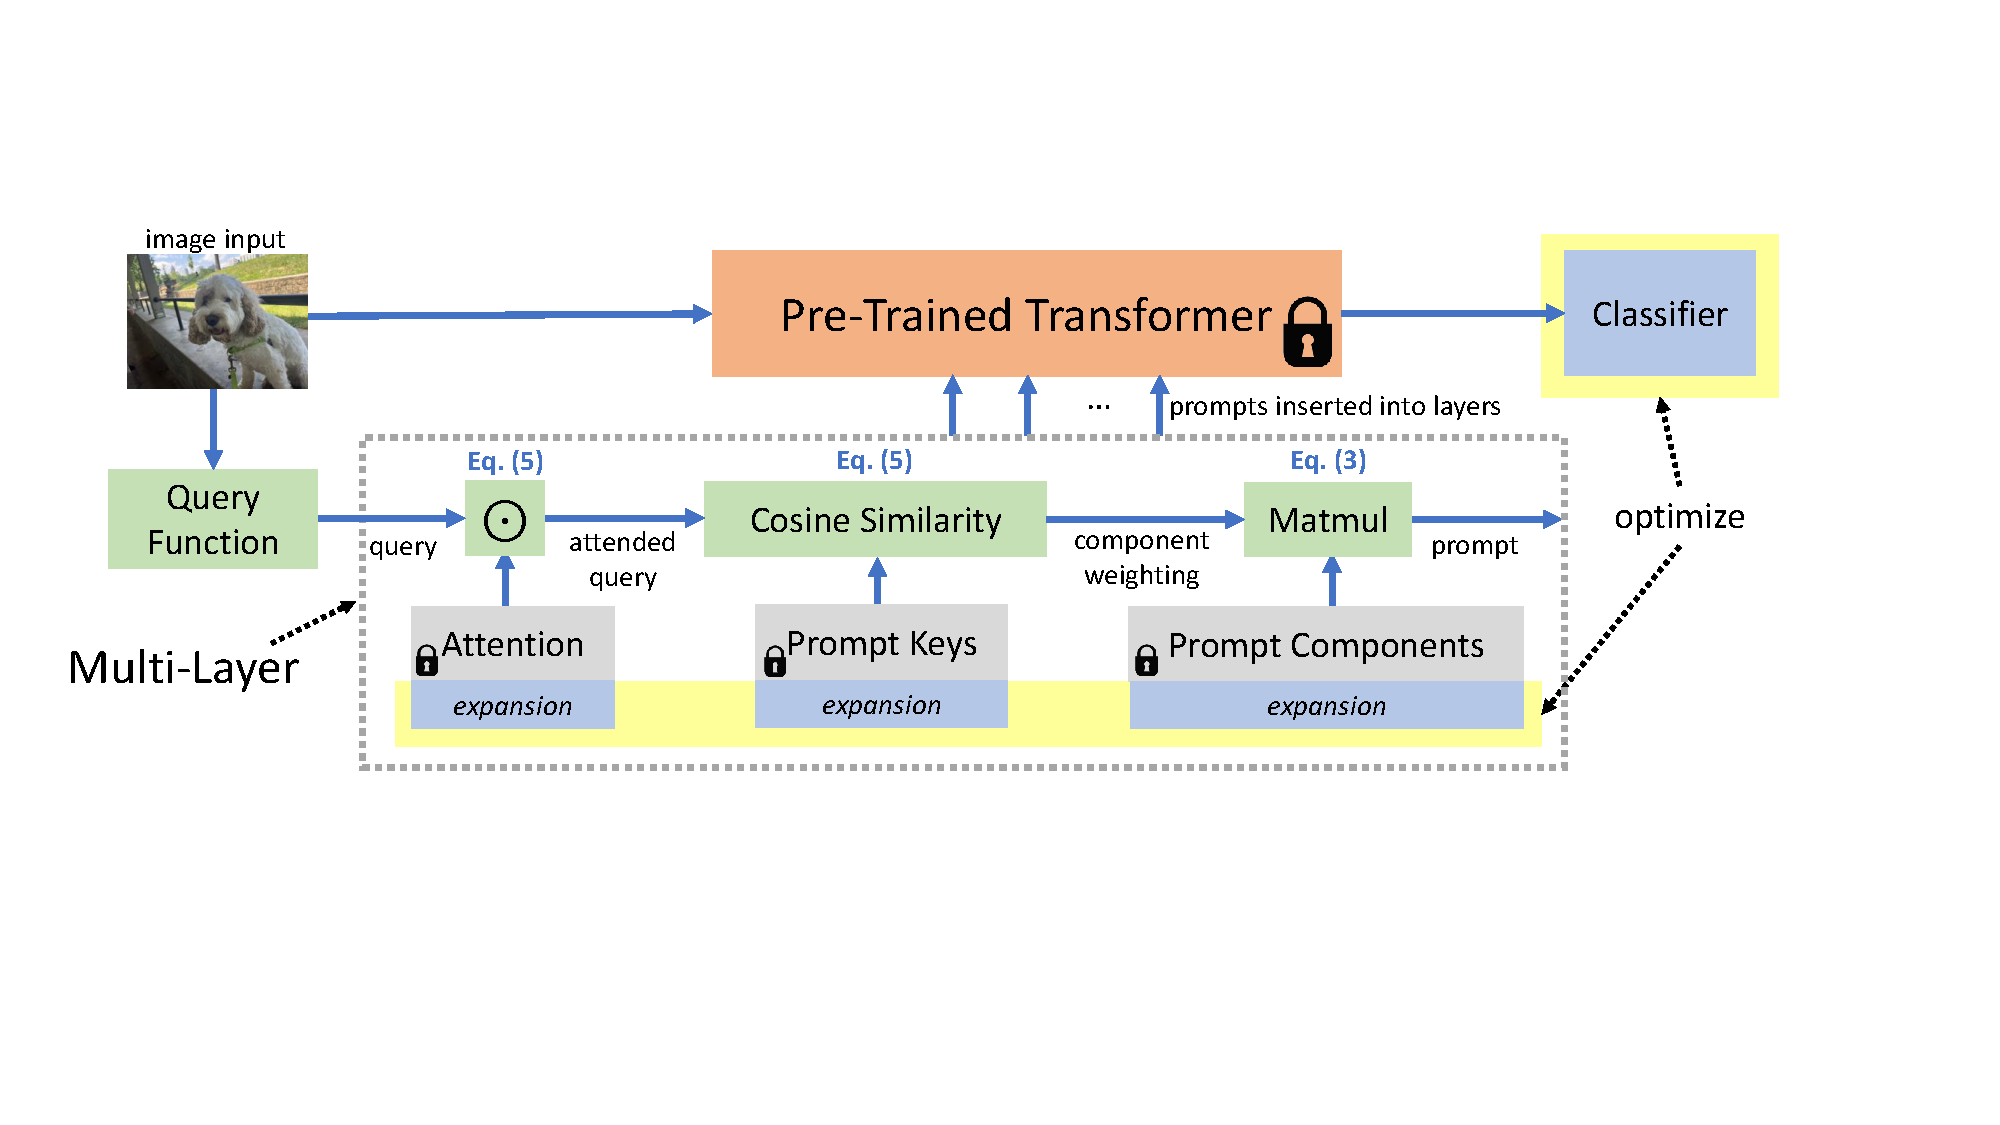
\includegraphics[clip, trim=1.2cm 6cm 3.8cm 3.6cm, width=0.95\textwidth]{figures/source/approach-new.pdf}
    \caption{\textbf{Our CODA-Prompt approach to rehearsal-free continual learning}. An input (e.g., image) is passed through a query function (we use the pretrained ViT encoder) and used for a novel \textbf{attention-based prompt-selection scheme} to produce prompts which are passed to multiple layers of a large-scale, pre-trained transformer. Our method is parameterized by an \emph{expanding} set of small prompt components, with each prompt having a corresponding key and attention vector. Both the input and produced prompts are passed through the transformer and sent to the task head. Only the prompting and task parameters are learned which is \emph{parameter efficient} and no training data is stored for replay which is \emph{memory-efficient and privacy preserving.} \emph{Importantly, our prompt selection scheme can be optimized end-to-end, unlike prior works which have a local similarity-based optimization for key-query matching.}
    }
    \label{fig:method}
    \vspace{-3mm}
\end{figure*}




\subsection{Prompt Formation}

While prompting has been shown to perform exceptionally well in terms of mitigating catastrophic forgetting, the existing state-of-the-art approach DualPrompt lacks the ability to expand learning capacity within a given task. Specifically, DualPrompt learns a \emph{single prompt} for each new task - regardless if the task is easy (such as learning a handful of new object classes) or complex (such as learning a large number of new object classes). One might try to increase the length of the prompt, but we show in our experiments (Section~\ref{section:exp_ablations_analysis}) that increasing the prompt length has saturated returns. Intuitively, we instead desire a method where the learning capacity is correlated to the underlying complexity of task data, rather than a single prompt. Additionally, we desire an approach that is end-to-end differentiable, which we conjecture increases the ability to learn a new task with higher accuracy.

We grow our learning capacity by introducing a new axis: \emph{a set of prompt components}. Rather than pick and choose prompts from a pool, we learn a set of prompt components which, via a weighted summation, form a \emph{decomposed}\footnote{Decomposed in the sense that our prompt is a weighted summation of components.} prompt that is passed to the corresponding MSA layer. This allows us to grow our prompting capacity to arbitrary depth and capture the rich underlying complexity of any task while maintaining a fixed prompt length. In addition, prompting in new tasks will inherently reuse the previously acquired knowledge of past tasks rather than initializing a new task prompt from scratch. 

Specifically, we replace learnable prompt parameter $\bm{p}$ with a weighted summation over the prompt components:
\begin{equation}
\bm{p} = \sum_{m} \alpha_m \bm{P_m}
\label{eq:prompt_f}
\end{equation}
where $\bm{P} \in \mathbb{R}^{L_{p} \times D \times M}$ is our set of prompt components, $M$ is the length of our set (i.e., the introduced axis of additional capacity), and $\alpha$ is a weighting vector that determines the contribution of each component which will be discussed in the next subsection.

A distinct difference between our method and L2P/DualPrompt is that \emph{all of our learnable parameters are optimized using the classification loss} rather than splitting into two separate loss optimizations. This allows for better end-to-end learning in our method, and we argue this is a key reason why our method performs better in the benchmarks described in Section~\ref{sec:exp}.

\subsection{Prompt-Component Weighting}

Rather than a pool of prompts, we have a set of prompt components and desire to produce a \emph{weight vector} $\alpha$ given a query $\theta(x)$, rather than a prompt index. We compute the cosine similarity between a query and keys to produce our weighting vector as:
\begin{equation}
\begin{aligned}
\alpha &= \gamma(q(\bm{x}),\bm{K}) \\
&= \{ \gamma(q(\bm{x}),\bm{K}_1),\gamma(q(\bm{x}),\bm{K}_2),\ldots, \gamma(q(\bm{x}),\bm{K}_M)\}
\label{eq:prompt_weight_a}
\end{aligned}
\end{equation}
where $\bm{K} \in \mathbb{R}^{D \times M}$ contains keys corresponding to our prompt components. The intuition here is that the contributing magnitude of each prompt component $\bm{P_m}$ to the final prompt $\bm{p}$ is determined by the similarity between the query $q(\bm{x})$ and corresponding key $\bm{K_m}$.

The prompt-query matching can be thought of as clustering in a high dimension space 
$D$ which is a well-known and difficult problem~\cite{koppen2000curse}. To mitigate this drawback, we introduce another component to our key-query matching: \emph{attention}. Each $\bm{P_m}$ has a corresponding attention vector $\bm{A_m}$ in addition to the key $\bm{K_m}$. This allows the the query to focus on certain features from the high dimensional query $q(\bm{x})$ output - for example, a prompt component used for mammalian face features to classify dogs and cats would be able to focus on relevant query features such as eye placement and skin texture, and furthermore ignore features of unrelated semantics, such as features useful for automobile classification. We use a simple feature-selection \emph{attention} scheme with element-wise multiplication between the query vector and attention vector to create an \emph{attended-query} which is then used for the key-similarity matching. Specifically, our updated approach to producing our weighting vector is:
\begin{equation}
\begin{aligned}
\alpha &= \gamma(q(\bm{x})\odot\bm{A},\bm{K}) \\
&= \{ \gamma(q(\bm{x})\odot\bm{A}_1,\bm{K}_1),\ldots, \gamma(q(\bm{x})\odot\bm{A}_M,\bm{K}_M)\}
\label{eq:prompt_weight_b}
\end{aligned}
\end{equation}
where $\bm{A} \in \mathbb{R}^{D \times M}$ contains learnable parameters (attention vectors) corresponding to our prompt components and $\odot$ is the element-wise product (also known as the Hadamard product). Notice that our attention vectors are learnable feature weightings rather than input-conditioned modules - we found that this fixed representation was less vulnerable to forgetting by its simple design, similar to the our prompt component keys.

\subsection{Expansion \& Orthogonality}
\label{sec:method_expand}

Crucial to mitigating catastrophic forgetting is the avoidance of \emph{overwriting} knowledge acquired in prior tasks. When we visit a new task we freeze our current components and expand the set, only updating the new components. This is visualized in the bottom of Figure~\ref{fig:method} where the existing parameters are \emph{locked} and only the expanded parameters are optimized. Specifically, in task $t$ we learn $\frac{M}{N}$ components where $N$ is the number of tasks and $M$ is a chosen hyperparameter, keeping the previous $\frac{(t-1) \cdot M}{N}$ components \emph{frozen}. This expansion is enabled by our attention-based component-weighting scheme, in that expanding our parameters do \emph{not} alter the computation of weights $\alpha$ corresponding previously learned components. For example, expanding the capacity of a nonlinear model like an MLP module, transformer attention head~\cite{dosovitskiy2020image}, or hyper-network~\cite{von2019continual} would alter the weight outputs of previously learned components. 

While the prior heuristic is focused on reducing catastrophic forgetting (not destroying previously acquired knowledge), we also want to reduce interference between existing and new knowledge. To do this, we add an orthogonality constraint to $\bm{P}$, $\bm{K}$, and $\bm{A}$. The intuition is that orthogonal vectors have less interference with each other. For example, we would want a key and prompt learned in task 2 to not attract task 1 data, otherwise the encoder output for task 1 data will change, resulting in misclassified data. We use an orthogonal initialization and introduce a simple orthogonality penalty loss to our method as:
\begin{equation}
\mathcal{L}_{ortho}(B) = ||B B^\top - I||_2
\label{eq:ortho}
\end{equation}
where $B$ represents any arbitrary matrix.


\subsection{Full Optimization}

Given task classification loss $\mathcal{L}$, our full optimization is:
\begin{equation} \label{eq:full_loss}
\begin{aligned}
    \underset{\bm{P^n}, \bm{K^n}, \bm{A^n}, \phi_{n}}{\operatorname{min}}  &\mathcal{L}(f_\phi(f_{\theta,\bm{P},\bm{K},\bm{A}}(\bm{x})), y) \quad + \\
    \lambda (\mathcal{L}_{ortho} &\left( \bm{P} \right) + \mathcal{L}_{ortho}\left( \bm{K} \right) + \mathcal{L}_{ortho}\left( \bm{A} \right) )
\end{aligned}
\end{equation}
where $\bm{P^n}, \bm{K^n}, \bm{A^n}$ refer to the prompt components and corresponding keys/attention vectors that are unfrozen and trained during task $n$ (see Section~\ref{sec:method_expand}) and $\lambda$ is a hyperparameter balancing the orthogonality loss. Note that we do not update the logits of past task classes, consistent with L2P and DualPrompt. We formally refer to our method as \textbf{CO}ntinual \textbf{D}ecomposed \textbf{A}ttention-based \textbf{P}rompting, or simply \textbf{CODA-P}.


